\let\negmedspace\undefined
\let\negthickspace\undefined
\documentclass[journal]{IEEEtran}
\usepackage[a5paper, margin=10mm, onecolumn]{geometry}
%\usepackage{lmodern} % Ensure lmodern is loaded for pdflatex
\usepackage{tfrupee} % Include tfrupee package

\setlength{\headheight}{1cm} % Set the height of the header box
\setlength{\headsep}{0mm}     % Set the distance between the header box and the top of the text

\usepackage{gvv-book}
\usepackage{gvv}
\usepackage{cite}
\usepackage{amsmath,amssymb,amsfonts,amsthm}
\usepackage{algorithmic}
\usepackage{graphicx}
\usepackage{textcomp}
\usepackage{xcolor}
\usepackage{txfonts}
\usepackage{listings}
\usepackage{enumitem}
\usepackage{mathtools}
\usepackage{gensymb}
\usepackage{comment}
\usepackage[breaklinks=true]{hyperref}
\usepackage{tkz-euclide} 
\usepackage{listings}
% \usepackage{gvv}                                        
\def\inputGnumericTable{}                                 
\usepackage[latin1]{inputenc}                                
\usepackage{color}                                            
\usepackage{array}                                            
\usepackage{longtable}                                       
\usepackage{calc}                                             
\usepackage{multirow}                                         
\usepackage{hhline}                                           
\usepackage{ifthen}                                           
\usepackage{lscape}
\usepackage{circuitikz}
\tikzstyle{block} = [rectangle, draw, fill=blue!20, 
    text width=4em, text centered, rounded corners, minimum height=3em]
\tikzstyle{sum} = [draw, fill=blue!10, circle, minimum size=1cm, node distance=1.5cm]
\tikzstyle{input} = [coordinate]
\tikzstyle{output} = [coordinate]


\begin{document}

\bibliographystyle{IEEEtran}
\vspace{3cm}

\title{1.4.14}
\author{AI25BTECH11039-Harichandana Varanasi}
 \maketitle
% \newpage
% \bigskip
{\let\newpage\relax\maketitle}

\renewcommand{\thefigure}{\theenumi}
\renewcommand{\thetable}{\theenumi}
\setlength{\intextsep}{10pt} % Space between text and floats


\numberwithin{equation}{enumi}
\numberwithin{figure}{enumi}
\renewcommand{\thetable}{\theenumi}


\title{Solution: Collinearity Problem}
\author{AI25BTECH11039 -- Harichandana Varanasi}
\date{}

\begin{document}
\maketitle

\textbf{Question:}  
The points $A(-6,10)$, $B(-4,6)$ and $C(3,-8)$ are collinear.  
If $AB = \tfrac{2}{9}AC$, find the ratio $AB:BC$.

\bigskip
\textbf{Solution:}

\begin{align}
\vec{A} &= \myvec{-6\\10},\quad
\vec{B} = \myvec{-4\\6},\quad
\vec{C} = \myvec{3\\-8}
\end{align}

Let $\vec{B}$ divide $\vec{A}\vec{C}$ in the ratio $k:1$.
\begin{align}
\vec{B} &= \frac{k\vec{C}+\vec{A}}{k+1}
\end{align}

Also,
\begin{align}
k(\vec{B}-\vec{C}) &= \vec{A}-\vec{B}
\end{align}

Hence,
\begin{align}
k &= \frac{(\vec{A}-\vec{B})^\top(\vec{B}-\vec{C})}{\|\vec{B}-\vec{C}\|^2}
\end{align}

Now,
\begin{align}
\vec{A}-\vec{B} &= \myvec{-6\\10}-\myvec{-4\\6} = \myvec{-2\\4} \\
\vec{B}-\vec{C} &= \myvec{-4\\6}-\myvec{3\\-8} = \myvec{-7\\14} \\
\|\vec{B}-\vec{C}\|^2 &= (-7)^2 + (14)^2 = 245
\end{align}

\begin{align}
k &= \frac{\myvec{-2\\4}^\top\myvec{-7\\14}}{245} \\
  &= \frac{(-2)(-7) + (4)(14)}{245} \\
  &= \frac{14+56}{245} \\
  &= \frac{70}{245} = \frac{2}{7}
\end{align}

Therefore,
\begin{align}
AB:BC = 2:7,\qquad \frac{AB}{AC} = \frac{2}{9}.
\end{align}

Verification:
\begin{align}
\vec{B} &= \frac{7\vec{A}+2\vec{C}}{9} \\
        &= \frac{7\myvec{-6\\10}+2\myvec{3\\-8}}{9} \\
        &= \frac{\myvec{-42\\70}+\myvec{6\\-16}}{9} \\
        &= \frac{\myvec{-36\\54}}{9} \\
        &= \myvec{-4\\6}
\end{align}

Thus, the given $\vec{B}$ lies on $\vec{A}\vec{C}$ with the required ratio.
\noindent\textbf{3D Diagram:}
\begin{figure}[h!]
\centering
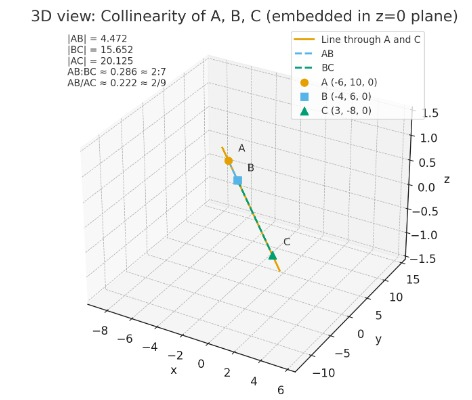
\includegraphics[width=0.7\linewidth]{figs/matgeo-1.4.14.jpeg}
\caption{3D view (embedded in $z=0$ plane) confirming collinearity}
\end{figure}

\end{document}

\end{document}